\section{Negative Selection Algorithm}

\begin{frame}
\begin{center}
\begin{spacing}{2.0}
 \Huge {Negative Selection Algorithm}
 \large {\\Li, Meizhen}
\end{spacing}
\end{center}
\end{frame}


\begin{frame}{Inspiration-Biological immune system}
  \begin{itemize}
  \item {
    The antigen-antibody reaction is an exclusive process.
  }
  \item {
    The primary role of immune system is to distinguish self from non-self.
  }
  \item {
    Immune cells are tolerant to self antigens but activate defense mechanisms when recognize non-self antigens.   
  }
  \item {
    The negative selection of T cells happened in the thymus during maturation.
  }
  \end{itemize}
\end{frame}

\begin{frame}{Biological immune system}
  \begin{figure}[hb]
  \centering
  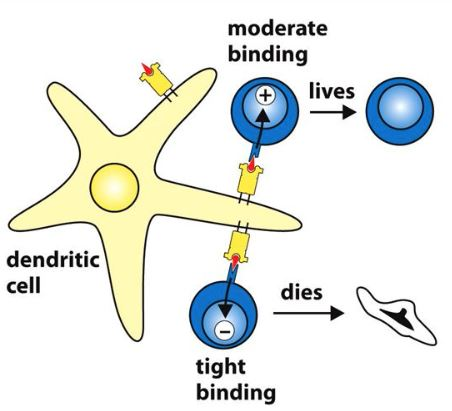
\includegraphics[width=0.6\textwidth]{img/NST.JPG}
  \caption{Negative selection of T cells}
  \end{figure}
\end{frame}

\begin{frame}{Biological immune system}
  \begin{figure}[hb]
  \centering
  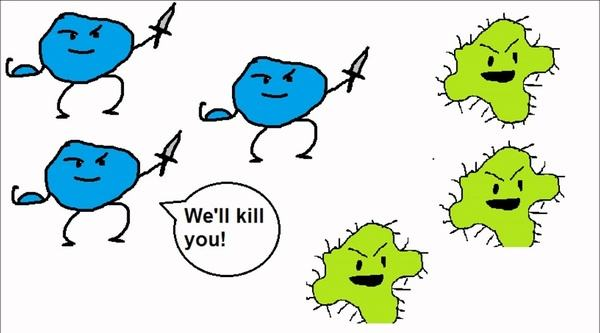
\includegraphics[width=0.6\textwidth]{img/ag_ab.jpg}
  \caption{Antigen-antibody interaction}
  \end{figure}
\end{frame}

% You can reveal the parts of a slide one at a time
% with the \pause command:
\begin{frame}{Defining the NSA}
  \begin{itemize}
  \item<1->{
    Define Self as a normal pattern of activity or stable behavior of a system/process.\\
    -Represent the collection as multiset of S of strings of length \emph{l} over a finite alphabet.
  }
  \item<2-> {   
    Generate a set R of detectors,each of which fails to match any string in S.
  }
  % You can also specify when the content should appear
  % by using <n->:
  \end{itemize}
\end{frame}
 
\begin{frame}{Flowchart}
  \begin{figure}[hb]
  \centering
  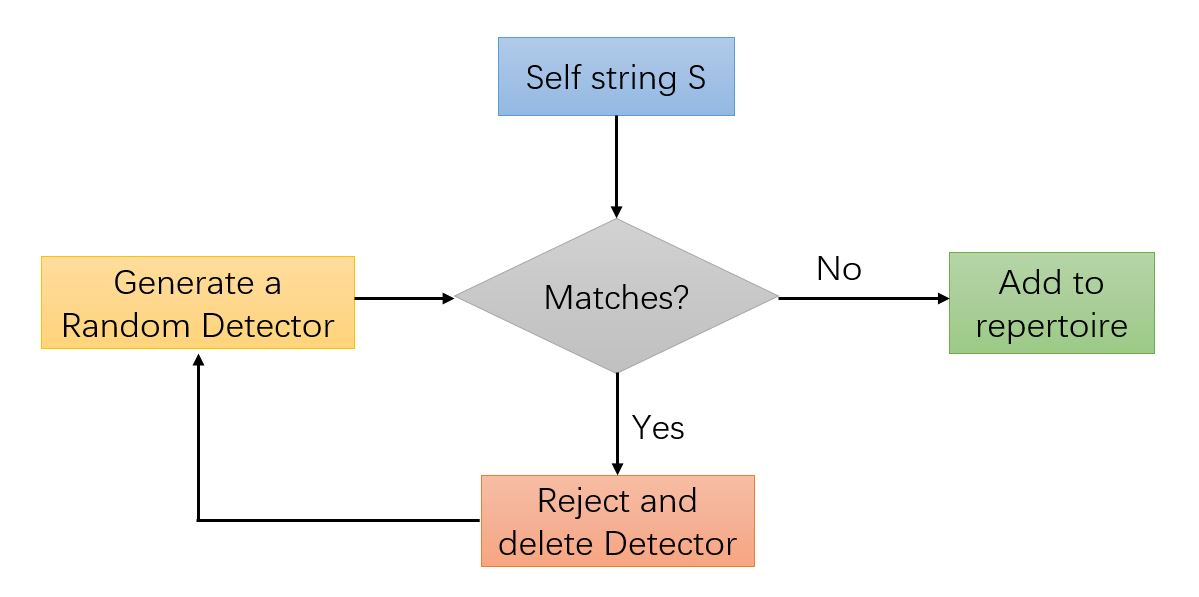
\includegraphics[width=0.8\textwidth]{img/NSAflowchart1.jpg}
  \caption{Generation of effective detector}
  \end{figure}
\end{frame}

\begin{frame}{Pseudocode}
 \begin{algorithm}[H]
  \caption{Detector Generation}          
  \label{alg1}      % and a label for \ref{} commands later in the document
    \begin{algorithmic}  
       \STATE Input:SelfData
       \STATE Output:Repertoire
       \STATE Repertoire $\Leftarrow$ emptyset
       \WHILE {$ !StopCondition()$}
       \STATE Detectors $\Leftarrow$ GenerateRandomDetectors()
       \FOR {Detector[i] $\in$ Repertoire }
       \IF {$not$ Matches(Detector[i],SelfData)}
       \STATE Repertoire $\Leftarrow$ Detector[i]
       \ENDIF
       \ENDFOR
       \ENDWHILE
       \STATE Return (Repertiore)

    \end{algorithmic}
  \end{algorithm} 
\end{frame}

\begin{frame}{Defining the NSA}
  \begin{itemize}
  \item {
    Monitor new observations for changes by continually testing the detectors matching against representatives of S.  If any detector ever matches, a change must have occurred in system behavior.
  }
  \end{itemize}
\end{frame}

\begin{frame}{Flowchart}
  \begin{figure}[hb]
  \centering
  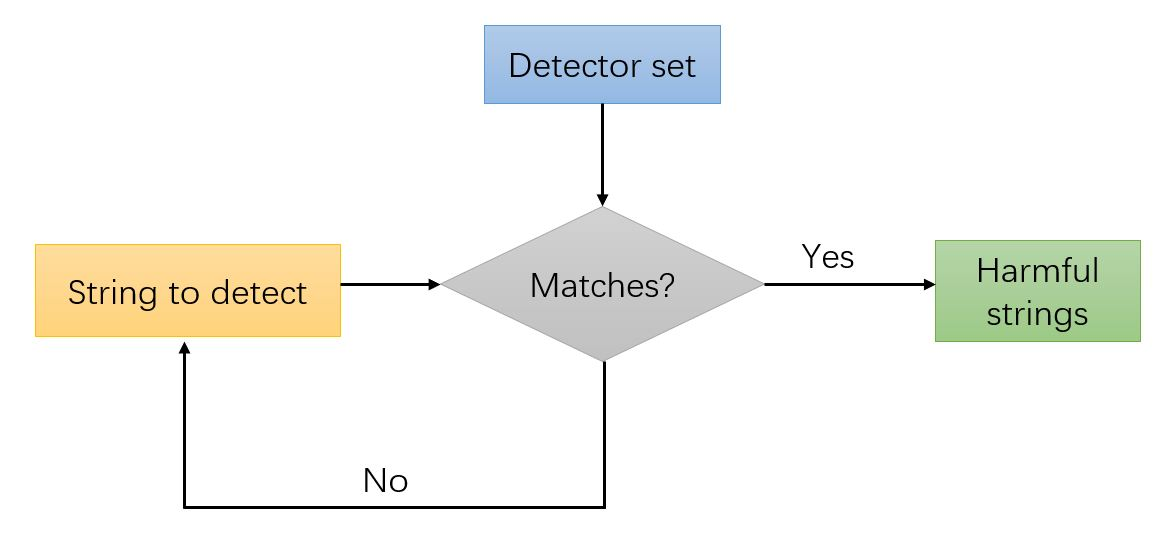
\includegraphics[width=0.8\textwidth]{img/NSAflowchart2.jpg}
  \caption{Detector application}
  \end{figure}
\end{frame}

\begin{frame}{Pseudocode}
 \begin{algorithm}[H]
  \caption{Detector Monitering}          
  \label{alg2}      
    \begin{algorithmic}  
       \STATE Input:InputSamples,Repertoire
  
       \FOR {Input[i] $\in$ InputSamples}
       \STATE Inputiclass $\Leftarrow$ nonself  
       \FOR {Detector[j] $\in$ Repertoire }
       \IF {Matches(Detector[j],SelfData)}
       \STATE Inputiclass $\Leftarrow$ self
       \ENDIF
       \ENDFOR
       \ENDFOR            
    \end{algorithmic}
  \end{algorithm} 
\end{frame}

\begin{frame}{Mathematical description}
 \begin{algorithm}[H]
  \caption{Define parameters}          
 % \label{alg3}      
    \begin{algorithmic}  
       \STATE N$_{R_0}$:number of initial detectors
       \STATE N$_{R}$:number of mature detectors 
       \STATE N$_{S}$:number of self elements
       \STATE P$_{M}$:random match probability at specific condition
       \STATE P$_{f}$:failed match probability
       \STATE f:the possibility of a random string not matching Selfset
    \end{algorithmic}
  \end{algorithm} 
\end{frame}

\begin{frame}{Mathematical description}
  \begin{equation}
     P_{Detectors}: f=(1-P_{M})^{N_{S}}
  \end{equation}
  \begin{equation}
     FailedMatch:P_f=(1-P_{M})^{N_{R}}
  \end{equation}
  \begin{equation}
     Detector:N_R=\frac{lnP_f}{ln(1-P_M)}
  \end{equation}
  \begin{equation}
     Iterations:D=\frac{lnP_f}{(1-P_{M})^{N_{S}}ln(1-P_M)}
  \end{equation}
  
\end{frame}

\begin{frame}{Optimization-detector generation}
   \begin{itemize}
      \item {
    Linear time detector generating algorithm
      \begin{equation}
        TimeComplexity=O((l-r)\times{N_S})+O((l-r)\times{2^r})+O(l\times{N_R})
      \end{equation}
    }
      \item {
    Greedy detector generating algorithm
     \begin{equation}
        TimeComplexity=O((l-r)\times{N_S})+O((l-r)\times{2^r}\times{N_R})+O(l\times{N_R})
     \end{equation}
    }
  \end{itemize}
\end{frame}


\begin{frame}{Optimization-detection time complexity}
  \begin{itemize}
  \item{
     Detection time complexity has linear corelation with N$_R$\\
  \begin{equation}
     Detector:N_R=\frac{lnP_f}{ln(1-P_M)}
  \end{equation}  
  \begin{equation}
     P_Mcontinous \approx \frac{1}{2^r}[\frac{l-r}{2}+1]
  \end{equation}
  \begin{equation}
     P_Mhamming = \frac{1}{2^r}\sum_{i=r}^{n}C_l^i
  \end{equation}
 }
  \end{itemize}
\end{frame}

\begin{frame}{Optimization-detection time complexity}
  
  \begin{figure}[hb]
  \centering
  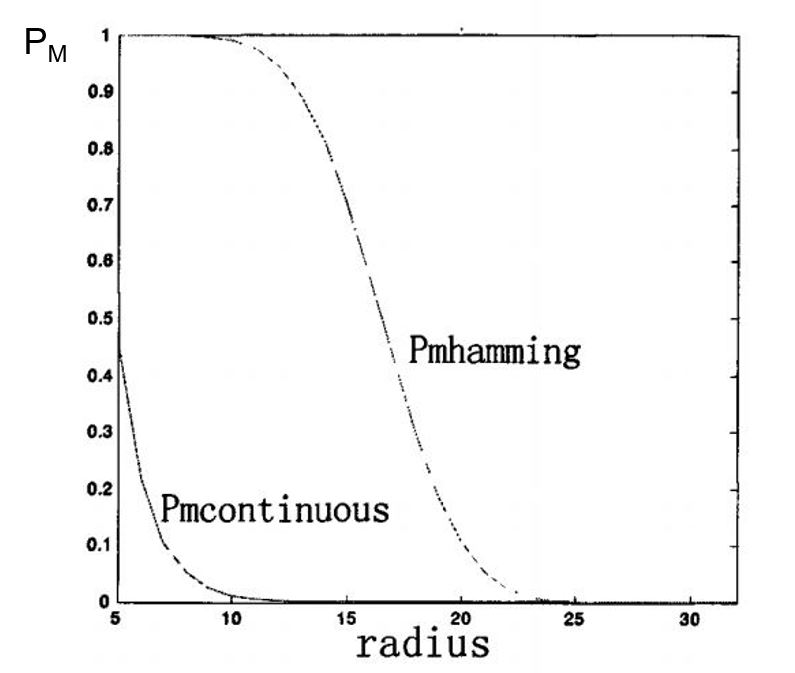
\includegraphics[width=0.6\textwidth]{img/CompareCH.jpg}
  \caption{With a specified r,P$_{Mcontinous}$ $\textless$ P$_{Mhamming}$,N$_{Rcontinous}$ $\textgreater$ N$_{Rhamming}$}
  \end{figure}
\end{frame}

\begin{frame}{Define black hole}
  \begin{figure}[hb]
  \centering
  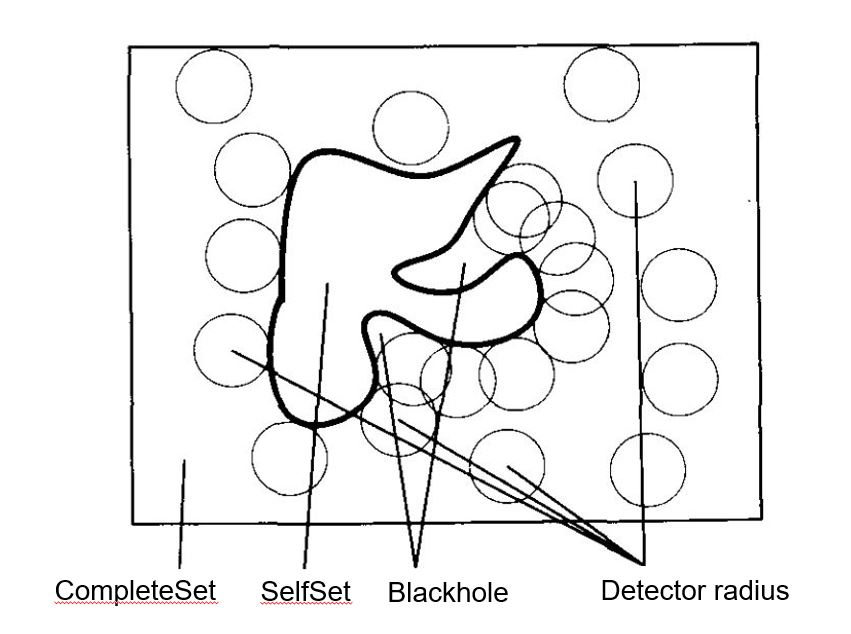
\includegraphics[width=0.6\textwidth]{img/blackhole.jpg}
  \caption{Definition of black hole}
  \end{figure}
\end{frame}

\begin{frame}{Reduce black hole}
   \begin{algorithm}[H]
   \caption{r-adjustable negative selection algorithm}          
 % \label{alg3}      
    \begin{algorithmic}  
       \STATE Step1: Define SelfSet S (length=l) r$_1$,r$_2$,...,r$_c$
       \STATE Step2: a $\Leftarrow$ GenerateRandomString (length=l) r=r$_1$
       \STATE Step3: Matches (a,S[i])
       \IF {$not$ Matches(a,S[i])}
       \STATE go to step2
       \ELSIF {r \textgreater r$_c$}
       \STATE go to step2
       \ELSE
       \STATE r=r$_{++}$ 
       \STATE go to step3
       \ENDIF 
       
    \end{algorithmic}
  \end{algorithm} 
\end{frame}

\begin{frame}{Reduce black hole}
  \begin{figure}[hb]
  \centering
  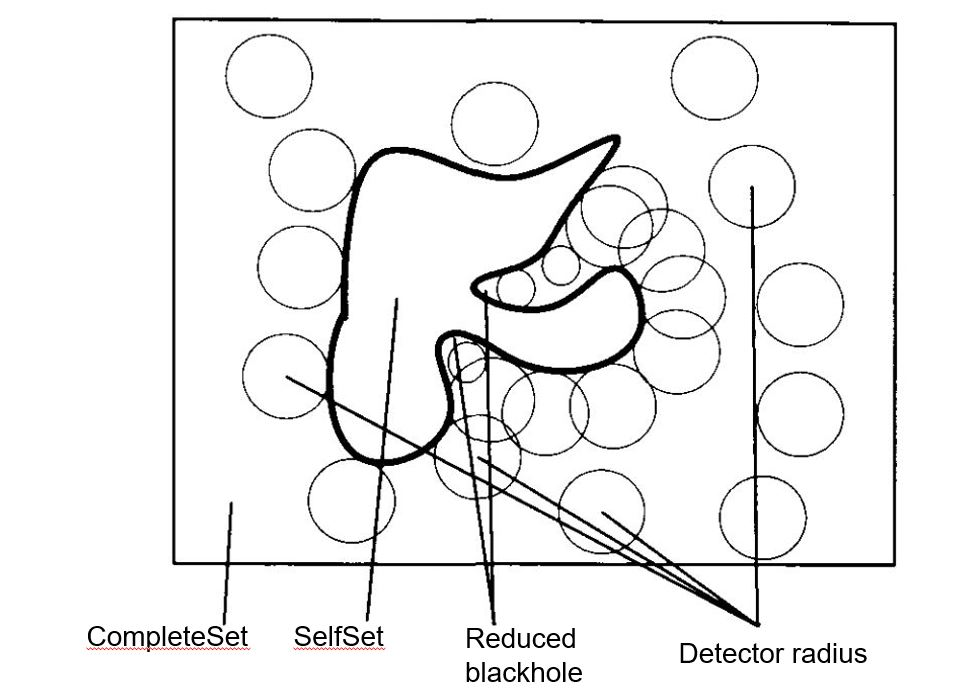
\includegraphics[width=0.6\textwidth]{img/reducedblackhole.jpg}
  \caption{the number of blackhole and iteration to generate mature detector have reduced}
  \end{figure}
\end{frame}

\begin{frame}
\begin{center}
\begin{spacing}{2.0}
 \Huge {Thanks}
 \large {\\Li, Meizhen}
\end{spacing}
\end{center}
\end{frame}
